     %%%%%%%%%%%%%%%%%%%%
     %                  %
     %  capitolo1.tex   %
     %                  %
     %%%%%%%%%%%%%%%%%%%%

\section{Sviluppo dell'applicativo}\label{sec:software}

\subsection{Obiettivi}
L' obiettivo del software è quello di realizzare un applicativo che esegua \textit{model based tracking} (vedi sezione \ref{modelTracking}) sulla base di un video passatogli come ingresso. Più nel dettaglio l'applicazione esegue il tracciamento tramite il filtro di Kalman \cite{kalman-intro} e il ConDensation \cite{kalman-condense}, in maniera tale da poter confrontare le prestazioni dell' uno e dell'altro.\\
Altri requisiti funzionali sono quelli di:

\begin{itemize}
 \item  fare scegliere all'utente l'oggetto da tracciare in caso di tracking multiplo: in questo caso il software si ferma sul primo frame del video, dando possibilità di scegliere l'oggetto di cui si vuol fare il tracciamento. Per migliorare la selezione di un oggetto, vengono evidenziati dei puntini gialli in corrispondenza dei blob identificato. Vedi figura \ref{fig:scelta2blob}

\item tracciare a video l'andamento dei due algoritmi, evidenziandoli con colori differenti; visualizzare un' ellissi per ogni algoritmo che indichi la varianza del vettore di stato per quel tipo di tracking.

\item fornire un output razionalizzato su terminale e su filesystem per verificare rispettivamente la corretta esecuzione degli algoritmi e per avere un riscontro finale sulle performance e l'accuratezza di ognuno. Successivamente parsare i suddetti file per una rappresentazione grafica dell'accuratezza dei due metodi di tracking.

\item progettare e realizzare l'applicazione in maniera tale che possa essere compilata ed eseguite su piattaforme diverse.


\end{itemize}

I dettagli implementativi di questi punti sono rimandati alla sottosezione  \ref{ControlFlow}

\begin{figure}[hb]
\centering
	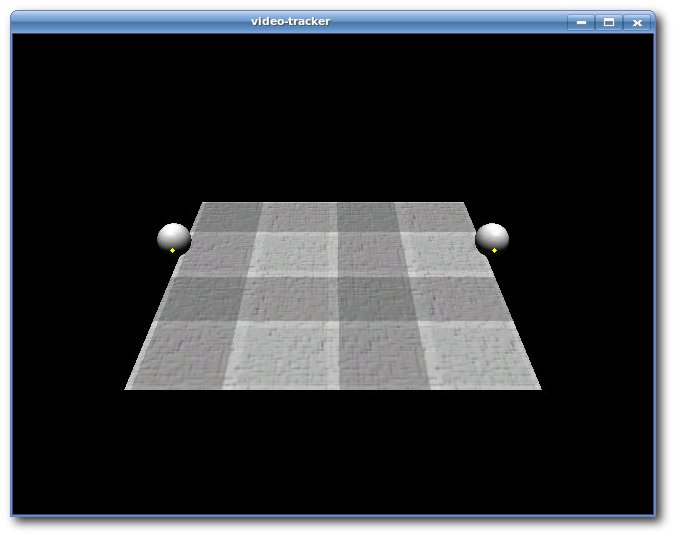
\includegraphics[scale=0.5]{doppiascelta.jpg}
\caption[Esempio di scelta tra due blob]{\textit{Esempio di scelta tra due blob su tracking multiplo: l'utente ha la possibilità di sccegliere su quale blob effettuare il tracciamento semplicemente cliccando vicino ad uno dei punti gialli. Il Sistema automaticamente selezionerà il blob più vicino attraverso il calcolo della distanza euclidea}\label{fig:scelta2blob}}
\end{figure}


\'E bene sottolineare che il video in ingresso possiede delle restrizioni; infatti affinchè il \textit{background subtraction} lavori in maniera ottima, è necessario che il video:
\begin{itemize}
 \item possieda semper uno sfondo fisso o che comunque non vari durante la ripresa. Cambiare sfondo sarrebbe come rinizializzare l'agoritmo per il detecting dei blob.
\item possieda un numero ( $n > 40 $ ) di frame inziale che mostrino solo il background per facilitare il calcolo della \textit{ground truth}, cioè del blob osservato da cui prendere le misure per i due algoritmi.
\item sia stato registrato da una postazione fissa e quindi che la telecamera di ripersa non introduca nel video un moto relativo.
 \end{itemize}

Qualsiasi video che rispetti questi tre vincoli è considerato non solo adeguato, ma ottimale per effettuare il tracking con la nostra applicazione.




%ingresso video fatto in un certo modo (sfondo fisso, tot frame di background iniziale, telecamera fissa)

%uno o + oggetti in moto

%permette di selezionare QUALE oggetto seguire, farne il tracciamento reale, ottenere le predizioni secondo k e c, e raccoglierne dati e risultati per la realizzazione di grafici

%intro utilizzo librerie utilizzate intel openCV
\subsection{Librerie Intel OpenCV}
Per svilluppare l'applicazione sono state utilizzate le librerie \textit{OpenCV} (Open Source Computer Vision), emergente nel campo della \textit{computer vision}  e sviluppata da Intel sotto una licenza di tipo OpenSource, compatibile con la GNU GPL.
\'E bene però prima fare chiarezza sull'uso e lo scopo di queste librerie.\\

La capacità di interpretare ed utilizzare correttamente le informazioni acquisite da una videocamera o fotocamera attualmente presenta molti problemi insoluti. Convertire un’immagine in informazioni “oggettive” astraendone il contenuto dalla pura rappresentazione luminosa, sebbene sia un’operazione banale per un cervello umano adulto è, a tutt’oggi, un problema di elevata complessità per un sistema automatico.
Oltretutto il campo di ricerca è evidentemente molto giovane, con meno di trent’anni di esperienza. In quest’ottica si inserisce la necessità di una base comune di potenti strumenti analitici, primo dei quali una \textbf{libreria} che raccolga le funzionalità degli algoritmi più utilizzati e citati in letteratura, oltre che una serie di formati di rappresentazione dei dati secondo standard aperti e condivisi.\\

Le librerie OpenCV  nascono appunto a questo scopo; lo sviluppo prende le mossa da un gruppo di ricerca sponsorizzato da Intel. E’ infatti parzialmente basata sulla \textit{Intel Image Processing Library (IPL)}: tale prodotto è oggi integrato nella libreria commerciale IIPP (Intel Integrated Performance Primitives), con cui conserva piena compatibilità e verso la quale rende disponibili un completo ventaglio di funzioni più specifiche.\\

Tra i punti di forza sottolineiamo inoltre la politica di licenza utilizzata, in stile BSD e definita nella ``Intel License Agreement For Open Source Computer Vision Library'', completamente compatibile con la licenza GPL. A grandi linee questo permette una libera ridistribuzione sia in forma sorgente che binaria, anche all’interno di prodotti commerciali, a condizione di mantenere le note di copyright e di non utilizzare il nome Intel a scopo promozionale di prodotti derivati.\\

Inoltre un' altra potenzialità offerta è la caratteristica di essere \textit{cross-platform}: cioè possono essere compilate e usate sia sotto sistema operativo Microsft Windows che GNU/Linux. Questa caratteristica le rende molto appetibili per i requisiti di portabilià che ci eravamo prefissi di raggiungere.\\ Da notare che le librerie sono scritte in linguaggio C e non fanno uso quindi di un linguaggio orientato agli oggetti.

\subsubsection{Aree funzionali delle librerie}\label{AreeFunz}
Si vuol chiarire subito un fatto che può essere causa di equivoci: con il termine ``libreria grafica'' infatti si identificano genericamente almeno tre famiglie di librerie, i cui scopi sono sostanzialmente differenti:
\begin{enumerate}
 \item  I Toolkit, ovvero librerie di primitive per la creazione di oggetti grafici di interfaccia (finestre, icone, bottoni,ecc). Parzialemente ricoperto in OpenCV dalle HighGui.
\item Librerie di rendering e multimedia, come DirectX e OpenGL, orientate alla massima performance nella creazione di effetti poligonali o vettoriali. L’utilizzo più comune è teso all’ottenimento di elevate prestazioni    grafiche sfruttate ad esempio nei videogiochi o nelle applicazioni multimediali.
\item  Librerie di gestione hardware grafico, come digitalizzatori e frame-grabber. Pur includendo tipicamente una base di funzioni di trattamento sono generalmente da considerarsi come API dei relativi driver hardware.
\end{enumerate}

Le OpenCV, pur includendo alcune funzionalità tipiche di ciascuna delle famiglie citate \footnote{vedi esempio delle HighGui}, non fanno parte di nessuno di questi gruppi. L’utilizzo primario è infatti quello collegato alla visione artificiale, il cui problema principale, come già visto, è quello di estrarre da immagini/video dati significativi, trattabili in modo automatico. Tale campo di studio trova le sue applicazioni più comuni nella robotica, nei sistemi di  videosorveglianza evoluti e nei sistemi di monitoraggio e sicurezza, oltre che in ogni sistema di archiviazione automatica di informazioni visive.\\

La libreria include attualmente più di 300 funzioni, che coprono le più svariate esigenze di trattamento di immagini, comprese funzioni matematiche ottimizzate (elevamento a potenza, logaritmi, conversioni cartesiane-polari, ecc.) ed  un completo pacchetto di algebra matriciale, sviluppato funzionalmente al resto del sistema.\\

La principale categoria di uso rimane comunque il processing di tipo real-time su immagini e video. \\
Una panoramica generale delle librerie comprende questi aspetti della computer vision:
\begin{enumerate}
\item Human-Computer Interface (HCI)
\item Object Identification
\item Segmentation and Recognition
\item Face Recognition e Gesture Recognition
\item Motion Tracking
\end{enumerate}

%descrivere un po queste aree e dove si usano noi nel nostro progetto.




\subsubsection{Riferimenti}

Come molti progetti opensource in maturazione \footnote{La versione 1.0 ufficiale è stata rilasciata nel tardo 2006; parte del progetto è stato scritto con librerie in beta testing} è stata carente la parte che riguarda la documentazione. Nonostante la presenza di un colosso alle spalle e di una struttura basata sul modello wiki, la documentazione ufficiale in pdf e html, anche se facilmente fruibile, non è stata sufficiente per colmare le lacune iniziali. Per questo motivo è stato effettuato un grosso lavoro di studio per capire il funzionamento del toolkit OpenCv, che spesso è terminato con la ricerca di documentazione in website asiatici, dove sembra che queste librerie siano molto gradite.\\
Alcuni riferimenti importanti per OpenCV:
\begin{itemize}
 \item \htmladdnormallink{Sito web ufficiale}{http://www.intel.com/technology/computing/opencv/index.htm} \cite{opencv}
\item \htmladdnormallink{Portale di wiki}{http://opencvlibrary.sourceforge.net} \cite{opencvwiki}
\item \htmladdnormallink{ OpenCv - Groups Community}{http://tech.groups.yahoo.com/group/OpenCV/} \cite{opencvgroups}
\end{itemize}


\subsection{Control Flow del programma}\label{ControlFlow}
%intro del ciclozzo FOR e che cosa viene fatto in ordine con l'acquisizione frame/frame del video
Come citato precedentemente, si va ora a evidenziare quelli che sono stato gli accorgimenti tecnici per implementare il nostro software di comparazione tra Kalman e Condensation.\\
Si cerca di non riportare tutto il codice sorgente, ma di evidenziare solo spezzoni di esso, che possono fornire preziose informazioni sulla struttura. \'E bene sottolineare che in linea con le OpenCV, la parte principale del software non è stata sviluppata secondo il paradigma Object Oriented, ma si è usato la creazione di strutture dati sottoforma di classi solo quando necessario.
Il nucleo centrale dell' applicazione è il \textbf{ciclo for}, il quale dipende dalla lunghezza del video da analizzare. Ogni passo di computazione verrà fatto in \textbf{modalità online}, cioè ad ogni passo dentro il ciclo stesso, in maniera incrementale. In questo senso nessuno dei passi che andiamo a eseguire per fare il tracking risulta avere priorità su altri. \footnote{Per meglio spiegare gli effetti del metodo online si suppone di effettuare fuori dal ciclo il background subtraction su tutto il video e una volta finito questo passare all'analisi. Così facendo si appesantisce tutto l'algoritmo di calcolo e si fornisce una lunga e inutile attesa lato utente} \\


Gli \textit{steps} effettuati durante l'esecuzione del software sono i seguenti:
\begin{itemize}
\item Apertura del video da filesystem e ottenimento delle informazioni
\item Ciclo su tutti frame del video:
	\begin{enumerate}
	\item Background Subtraction
	\item Aggiornamento di Kalman e Condensation
	\item Rappresentazione dei risultati 
	\end{enumerate}
\end{itemize}

Nel listato di pseudo codice sottostante è riportata l'idea dell'andamento dell'applicativo.


\lstset{language=c++}
\lstset{commentstyle=\emph}
\begin{lstlisting}[frame=r,caption=Nucleo dell'Applicazione - execute.cpp ,breaklines=true,basicstyle=\small]{Nucleo dell'Applicazione - execute.cpp}

void execute( file ){

	video = captureFromAvi( file )
	
	initBackgroundSubtraction( video )

	for( int fr = 1; frame = captureNextFrame( video ), fr++ ){
	
		updateBackgroundSubtraction( frame )
		
		if ( frame == FIRST_FRAME){
			
			blob = getBlobSelectedFromUser( frame )
	
			initKalman( blob );
			
			initCondensation( blob );
		}
		else{
		blob= getBlob(Frame);
		updateKalman(blob);
		updateCondensation(blob);
		}
	}
}



\end{lstlisting}

Successivamente analizzeremo solo alcuni dei precedenti \textit{steps} elencati.

\subsubsection{Back subtraction}\label{sec:bgsub}
%realizzazione online del backsub, librerie eccetera
L'idea di base del \textit{Background Subtraction}  è quella di identificare il livello di background per un determinato video, segmentando ogni frame in altri due frames chiamati rispettivamente:

\begin{itemize}
\item Foreground Mask
\item Background Mask
\end{itemize}



In letteratura vi sono diversi modelli e/o metodi per calcolare la segmentazione tra foreground/background. In particolare citiamo:
\begin{description}
 \item[Distribuzione Unimodale] Il più semplice modello assume che l'intensità del valore di un pixel può essere modellata da una distribuzione unimodale, come una distribuzione Gaussiana del tipo $N(\mu,\sigma^2)$
\item [Mixture of Gaussian MoG] Il modello MoG generalizzato viene di solito usato per modelli abbastanza complessi, non statici con molteplici background. Questo tipo di modellazione è di tipo statistico e online. L'idea è quella di modellare ogni pixel in un processo di funzioni gaussiane, successivamente eseguire l'apprendimento online e rilevare il foreground passo passo sulla base dell'intensità del valore di grigio di ogni pixel.
%Si eliman la gaussiana che ha minor peso e si aggiunge una nuova gaussiana con media uguale al valoredi quel pixel e varianza molto grande. Si aggiornano tutte le gaussiane e si normalizza...L’algoritmo di detection proposto è un algoritmo statistico, infatti, per la classificazione del pixel si considera la sua storia recente, rappresentata mediante un set di gaussiane: Mixture of Gaussians (MOG).
%La classificazione dei pixel viene effettuata stabilendo il matching di ogni pixel con le gaussiane ad esso associate: se non esiste matching il pixel viene classificato come foreground, se, invece, esiste matching, il peso della gaussiana corrispondente viene confrontato con un valore di soglia, se esso è minore di tale soglia il pixel viene ancora classificato come foreground, se è maggiore, viene considerato background.
In particolare un pixel sarà classificato come un pixel di foreground se la distribuzione a lui associata ha peso sufficientemente basso e varianza alta, viceversa verrà classificato come background pixel.
\item [Tecniche Non Parametriche] Si stima la funziona di densità di probabilità per ogni pixel preso dai tanti campioni, usando una tecnica di stima sulla densità di probabilità.
\item [Approccio basato su regioni o frame] \'E una tecnica basata su pixel, che assume che le serie di temi dell'osservazione è indipendente per ogni pixel. L'approccio ad alto livello è eseguito segmentando un'immagine in una regione o ridefinendo un sottolivello di classificazione ottenuto su ogni pixel.
 \end{description}

Nell'applicativo sarà usato il modello di Mixture of Gaussians (MoG), sia perchè si vuole coprire anche video di una certa complessità e sia perchè le librerie offrono un buon supporto per questo modello. In particolare nel listato sottostate è visualizzato l'uso di esse nel file addetto al background subtraction.

\lstset{language=c++}
\lstset{commentstyle=\emph}
\begin{lstlisting}[frame=r,caption=Background Subtraction implementato con MOG - getBackground.cpp ,breaklines=true,basicstyle=\small]{Background Subtraction implementato con MOG - getBackground.cpp}

///The function that init the Background subtraction with Gaussian model
/**
 * \param bgmodel the model strucutre
 * \param tmp_frame the temporary frame
 * \param bgmodel paramMog the parameters
 */

void initBackgroundModel(CvBGStatModel ** bgmodel, IplImage* tmp_frame, CvGaussBGStatModelParams* paramMoG){
	
	//Init of the params

	paramMoG->win_size = 200; 
	paramMoG->n_gauss = 3
	paramMoG->bg_threshold = 0.1;
	paramMoG->std_threshold = 5;
	paramMoG->minArea = 200.f;
	paramMoG->weight_init = 0.01;
	paramMoG->variance_init = 30; 
	
	//Init of the model

	*bgmodel = cvCreateGaussianBGModel(tmp_frame, paramMoG);
	
}


///The function that make the Background subtraction with Gaussian model
/**
 * \param aviName the name of the avi video to process
 * \return savedBackgroundImage the background of the video
 */

IplImage* updateBackground(CvBGStatModel *bg_model, IplImage * tmp_frame){
	 
	//Updating the Gaussian Model

	cvUpdateBGStatModel(tmp_frame, bg_model);
  
	
	//returing the binary background

	return bg_model->foreground;
}


\end{lstlisting}

Dalla prima funzione si nota come vengano inizializzati i parametri su cui poi sarà costruito il modello di previsione del foreground; in particolare si nota che:

\begin{itemize}
\item ogni pixel è classificato come processo che condivide 3 gaussiane 
\item la soglia ( il valore di grigio) per essere considerato background è settata a 0.1 
\end{itemize}
Per il resto del codice è giusto notare che ogni volta che si processa un nuovo frame anche l'algoritmo viene aggiornato su quel frame.

\begin{figure}[hbp]
\centering
	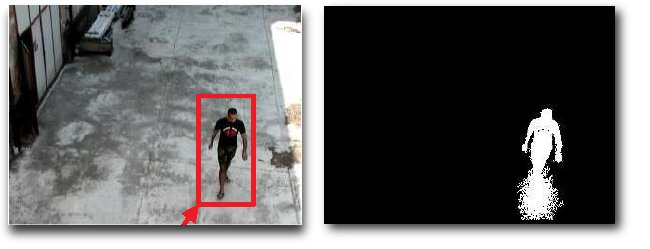
\includegraphics[scale=0.5]{bgsub.jpg}
\caption[Esempio di background subtraction graduale]{\textit{Esempio di background subtraction graduale. Viene segnalato nella prima finestra quello che è il foreground del video e in seguito nella seconda l'effetto del background subtraction che mette in rilievo il blob bianco rilevato sullo sfondo. Ovviamente come si vede nella figura se l'algoritmo non lavora in maniera ottimale è possibile ottenere blob che non esistono nell'immagine di partenza.}\label{fig:bgsub}}
\end{figure}
\newpage

\subsubsection{Predizione}
La parte di predizione dei dei due algoritmi è descritta nei file \texttt{kalman.cpp} e \texttt{condensation.cpp} ed è sufficientemente semplice, grazie all'astrazione fornita dalle librerie OpenCV.\\
Nel listato sottostante è rappresentato il passo di predizione del filtro di Kalman, già inizializzato , che effettua in sequenza:
\begin{enumerate}
 \item La predizione (\textit{Predict - Time Update}) del nuovo punto di stato sulla base del modello dinamico da noi descritto, cioè sulla base delle matrici A,B ed u.
\item La correzione (\textit{Correct - Measurament Update}) sul nuovo punto sulla base della misura ottenuta dalla \textit{ground truth} con il metodo del Background Subtraction. \'E da notare come nel vettore \texttt{measurement} vengono proprio inserite le componenti ottenute dall'osservazione.
\end{enumerate}

\lstset{language=c++}
\lstset{commentstyle=\emph}
\begin{lstlisting}[frame=r,caption=Predizione di Kalman - kalman.cpp ,breaklines=true,basicstyle=\small]{Predizione di Kalman - kalman.cpp}

///The function that will update the kalman structure with the data collected in extractBlob. it will provide to do the predict and the correct kalamn's step.
/**
 * \param kalman the pointer to the kalman structure
 * \param struct coordinate the struct in which are the measurement coordinate. (z_k)
 */

float* updateKalman(CvKalman * kalman, coord coord){
	
	int Meanx, Meany;
	CvMat* measurement = cvCreateMat(2,1, CV_32FC1 );
	Meanx = (int) coord.cX;
	Meany =  (int) coord.cY;
	cvmSet(measurement,0,0,Meanx);
	cvmSet(measurement,1,0,Meany);
	CvMat* u = cvCreateMat(1,1, CV_32FC1 );
	u->data.fl[0]=1;
	
	//Kalman Predict
	const CvMat* predict = cvKalmanPredict(kalman,u);

	//Kalman Correct
	const CvMat* correct= cvKalmanCorrect(kalman, measurement);
	
	return correct->data.fl;

}


\end{lstlisting}





Quanto detto è stato già ampiamente dimostrato nella sezione \ref{kalman} e in particolare nella figura \ref{fig:predictcorrect}; a livello di codice si nota che l'aggiornamento di Kalman è effettuato richiamando le funzioni \texttt{cvKalmanPredict(kalman,u)} e  \texttt{cvKalmanCorrect(kalman, measurement)}.\\
Infine è bene sottolineare che la predizione, come accordato nella \ref{sec:modelli}, è rappresentata da un vettore di due componenti, dove la prima rappresenta l'ascissa e la seconda l'ordinata nel piano del Video, che hanno come centro (0,0) il pixel in alto a sinistra.\\
\newpage
Lo studio che è stato effettuato per la descrizione del modello dinamico non è servito solo nel filtro di Kalman, ma è stato riusato anche nell'algoritmo del ConDensation. La matrice di transizione dello stato A, infatti è usata in esso per inizializzare ogni samples dell'algoritmo, generando i valori con un \textit{random seed} e limitandoli sulla base di due margini. Quanto detto è implementato nel listato sottostante nella funzione \texttt{initCondensation}.\\
Infine il processo di aggiornamento del condensation vede fondamentalmente due passi principali:
\begin{enumerate}
 \item l'aggiornamento delle varie probabilità per ogni samples inizializzato sulla base dell'osservazione ottenuta dalla \textit{ground truth}. Eseguito dall funzione \texttt{updateProcessProbDens}
\item  la scelta del sample a probabilità maggiore, operazione delegata dalla funzione presente in OpenCv dal nome \texttt{cvConDensUpdateByTime}
\end{enumerate}



\lstset{language=c++}
\lstset{commentstyle=\emph}
\begin{lstlisting}[frame=r,caption=Predizione di Condensation- condensation.cpp ,breaklines=true,basicstyle=\small]{Predizione di Condensation- condensation.cpp}

CvConDensation* initCondensation ( CvMat** indexMat, int nSample, int maxWidth, int maxHeight ){
	
	int DP = indexMat[0]->cols; //! number of state vector dimensions */
	int MP = indexMat[2]->rows; //! number of measurement vector dimensions */

	CvConDensation* ConDens = cvCreateConDensation( DP, MP, nSample );
	
	...

	for (int i=0;i<DP*DP;i++){
		ConDens->DynamMatr[i]= indexMat[0]->data.fl[i];
	}

	cvConDensInitSampleSet(ConDens, lowerBound, upperBound);
	
	CvRNG rng_state = cvRNG(0xffffffff);
	
	for(int i=0; i < nSample; i++){
		ConDens->flSamples[i][0] = cvRandInt( &rng_state ) % maxWidth;
		ConDens->flSamples[i][1] = cvRandInt( &rng_state ) % maxHeight;
	}

	
	return ConDens;
}

coord updateCondensation ( CvConDensation* ConDens, coord Measurement, float * stdDX_ptr, float * stdDY_ptr){
	coord prediction;
	
	updateProcessProbDens(ConDens, Measurement, stdDX_ptr, stdDY_ptr);
	
	cvConDensUpdateByTime(ConDens);
	
	prediction.set(ConDens->State[0], ConDens->State[1]);
	return prediction;	
}


\end{lstlisting}

\newpage
%\subsubsection{Rappresentazione della predizione}
\subsubsection{HighGui}
Come accennato nella sezione \ref{AreeFunz}, le librerie OpenCv offrono anche un parte di toolkit per realizzare semplici widget grafici in cui poter visualizzare immagini o video, oppure semplici form per incrementare/decrementare il tuning di determinati parametri. \'E bene sottolineare che esse permettono anche la gestione degli eventi lato utente; per esempio è possibile catturare eventuali click del mouse. Queste widget risultano molto utile ovviamente se si vuole che l'utente interagisca in maniera attiva con il software: nel nostro caso si è usato una semplice \textit{NamedWindow}, fornita da questo toolkit, in cui visualizzare il video con i relativi tracciamenti; in più si è creato un gestore di eventi per catturare eventuali click del mouse che permettono all'utente di selezionare il blob da tracciare in caso di tracking multiplo.
Il codice seguente mostra l'uso delle HighGui per realizzare quanto detto:

\lstset{language=c++}
\lstset{commentstyle=\emph}
\begin{lstlisting}[frame=r,caption=Uso delle HighGui - execute.cpp ,breaklines=true,basicstyle=\small]{Uso delle HighGui - execute.cpp}

//! Create the window

cvNamedWindow( "video-tracker", 1 );

...

if (frame == FIRSTFRAME) {

	cvSetMouseCallback( "video-tracker", on_mouse, 0);
	
	...

}

...

//! Display the temp frame in the window

cvShowImage("video-tracker", tmp_frame);

...


//! Left Click Mouse Event Functions

void on_mouse( int event, int x, int y, int flags, void* param ){
 
	switch( event ){
		case CV_EVENT_LBUTTONDOWN:{
		CLICK[0]=x;
		CLICK[1]=y;
		}break;
	}
}


\end{lstlisting}
\newpage
\subsubsection{Scripting GNUPlot}
Oltre lo sviluppo software, si è anche riusciti a salvare in output i risultati su file testuali, in modo tale da effettuare una successiva lettura con un qualsiasi visualizzatore di grafici com Excel o Matlab. I file prodotti contengono le coordinate, prese frame per frame, del blob stimato con il background subtraction e dei due tracciamenti. Inoltre è anche generato un file riassuntivo con i princiapli coefficieni di rendimento dei due metodi di tracking, quali varianza media e distanza media tra blob osservato e misurato.\\
Fatto ciò si è scelto il sistema libero GNUPlot per interpretare e dare una rappresentazione grafica automatizzata dei dati raccolti, con la possibilità di creare anche immagini su hardisk al volo dei grafici. Si è infatti prodotto uno scritp bash, (fruibile anche sui sistemi Windows con GNUPlot) ,che automatizza il \textit{processing} dell'output.\\
Lo script risulta il seguente:

\lstset{language=bash}
\lstset{commentstyle=\emph}
\begin{lstlisting}[frame=r,caption=Script bash che invoca GNUPlot con i vari file di configurazione - gplot.sh ,breaklines=true,basicstyle=\small]{Script bash che invoca GNUPlot con i vari file di configurazione - gplot.sh}
#!/bin/bash

gnuplot -persist plot-png > plot.png
gnuplot -persist plot-window 
gnuplot -persist plot-distances
gnuplot -persist plot-distances-png > plot-distances.png


\end{lstlisting}


\lstset{language=bash}
\lstset{commentstyle=\emph}
\begin{lstlisting}[frame=r,caption=Un esempio di file di configurazione dello scritp che visualizza il grafico - plot-window ,breaklines=true,basicstyle=\scriptsize]{Un esempio di file di configurazione dello scritp che visualizza il grafico - plot-window}
#gnuplitting scripiting

set key left below Right noreverse enhanced box linetype -1 linewidth 1.000 samplen 4 spacing 1 width 0 height 0 autotitles

set title 'Kalman and Condensation comparison'

set grid

plot 'coordinateKalman.txt' with point pt 1 , 'coordinateCondensation.txt' with point pt 1, 'coordinateReali.txt' with point pt 1



\end{lstlisting}

\begin{figure}[b]
\centering
	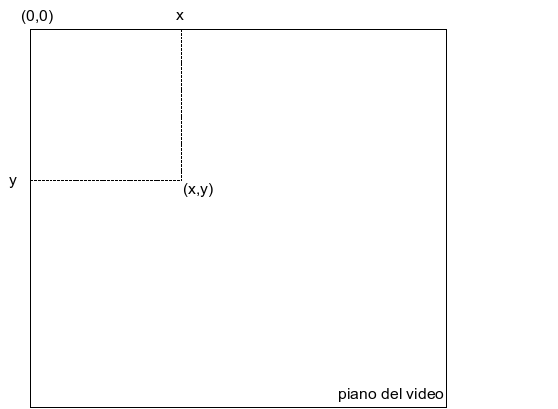
\includegraphics[scale=0.45]{piano.png}
\caption[Rappresentazione del vettore dello stato]{\textit{Rappresentazione del vettore dello stato}\label{fig:pianoStato}}
\end{figure}
